\section{State of the art}
    \subsection{Microbiome}
        % \subsubsection{Microorganism}
            Microorganisms also known as microbes are microscopic life forms. They pervade virtually every dimension of our planet. These tiny creatures exhibit a remarkable range of diversity. They include bacteria, archaea, fungi, protozoa, microalgae, and non-living viruses. And they are present in almost every environment on Earth. This includes soil, water, and air, as well as within and on the human body. Microbes play a vital role in maintaining ecological stability as they participate in processes like nutrient cycling, organic matter breakdown, and the formation of symbiotic connections with an array of other life forms. Furthermore, their influence on human health is substantial, with some microorganisms functioning as pathogens that induce disease, while others foster general well-being\cite{brock2003brock}.
    
            Since the advent of the microscope by Levenhoek, the investigation of microorganisms has been a continuous pursuit, leading to numerous scientific and technological advancements. Researchers have harnessed microbes for diverse objectives, including the generation of antibiotics, the enhancement of fermentation processes, and the development of groundbreaking biotechnologies. As our comprehension of microbes continues to evolve, their capacity to impact and improve numerous facets of human life and the environment is further magnified.
        
        % \subsubsection{Microbiome}
            The microbiome is the collective genome of all microorganisms that live in a given environment. The study of the microbiome is very important. To take the human microbiome as an example, the microbes that live in and on our bodies play a key role in maintaining homeostasis, influencing metabolism, and regulating the immune system. In fact, it is estimated that there are 10 times more microbial cells in the human body and that the combined (meta) genome of the microbes is more than 100 times the human genome \cite{yang2009more}.
            
            In recent years, the study of the microbiome has had more opportunities with advances in high-throughput sequencing technologies, which have made it possible to describe the details of microbial populations\cite{bharti2021current}. Researchers can now use technologies such as 16S ribosomal RNA (rRNA) gene sequencing,  Internal Transcribed Spacer (ITS) rRNA gene sequencing, and metagenomics to identify and quantify the microbes present in a given environment and their functional capabilities.
            
            Understanding the composition and function of the microbiome is important for a wide range of applications, from human health and disease to environmental protection and biotechnology to fermented foods, such as beer and wine. For example, researchers are investigating the role of the gut microbiome in diseases such as obesity, diabetes, and inflammatory bowel disease, and are exploring the potential of using microbiome-based therapies to treat these diseases\cite{durack2019gut}. In addition, the study of microbial communities in the environment is important for understanding ecosystem function and biodiversity, and for developing sustainable agricultural and industrial processes \cite{vuong2022little}. Many microbiomes are also involved in the production and fermentation of products such as beer, and understanding these microbiomes will be of great help in the development of fermentation for beer manufacturing.

    
    
    \subsection{Microbiome analysis}
            % In nature, a vast number of microorganisms exist, and only around 1\% of them are isolated and cultured \cite{martiny2019high}. Gaining a clear understanding of the composition and functional genes of microbial communities in environmental samples has long been a challenging issue. However, recent advancements in metagenomic technology through next-generation sequencing have improved the situation.

            % Metagenomics can be defined broadly or narrowly. Broadly, metagenomics encompasses the study of microbial community composition, functional genes, and metabolic products to reveal the structure and composition of microbial communities, as well as their interactions with hosts and within the community itself. Narrowly, metagenomics pertains to metagenomic DNA sequencing technology, which involves high-throughput sequencing of microbial community DNA to identify the types and abundance of all functional genes present in the community. This method consists of experimental and analytical stages, with the experimental stage primarily including sample collection, DNA extraction, and high-throughput sequencing. The data analysis stage primarily involves sequence quality control, assembly, gene prediction and quantification, community taxonomic profiling, and the comparison of differential functional genes and pathways between sample groups.
            
            % Metagenomics is a discipline rooted in technological advancements. Common techniques in this field are metabarcoding and shotgun sequencing.

 
        Microbiome analysis is a complex process that involves multiple steps from sample collection to data analysis. Each step and the different tools or protocols that can be used are outlined in this section.

        \begin{figure}[h]
            \centering
            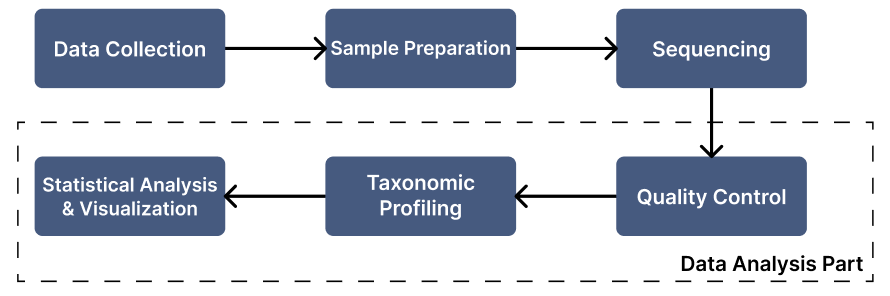
\includegraphics[scale=0.5]{images/state_of_the_art/microbiome_analysis.png}
            \caption{Common microbiome analysis steps}
            \small Microbiome analysis typically follows a structured methodology. The process begins with data collection, followed by sample preparation, sequencing, and ultimately, data analysis. The latter, as depicted by the dashed section in the figure, encompasses steps such as quality control, taxonomic profiling, as well as diversity analysis, and visualization. For methods like shotgun sequencing and metabarcoding, the tools used in the steps above can be different.
            \label{fig:state_of_art:microbiome_analysis}
        \end{figure}

        \paragraph*{Data collection}
        Sample collection is the first step in microbiome analysis and involves collecting samples from the environment of interest, such as soil, water, or host organisms. The use of appropriate sampling techniques is essential to maintain the integrity of the microbial community. Methods such as wiping, filtration, and direct sampling are commonly used and protocols vary depending on the sample type and study objectives.


        \paragraph*{Sample preparation}
        Sample preparation involves a series of procedures to prepare the collected samples for downstream high-throughput sequencing and analysis. Sample preparation encompasses processes that isolate and concentrate microbial DNA or RNA from complex sample matrices, convert it into a format suitable for sequencing, and generate libraries for high-throughput sequencing.

        For metabarcoding, which is also referred to as amplicon sequencing, the sample preparation process involves extracting genomic DNA from the collected samples, amplifying targeted DNA regions using PCR with specific primers (usually 16S rRNA gene for bacteria and ITS region for fungi), and preparing amplicon libraries for sequencing. This targeted approach enables the identification of specific taxa present in the sample, based on the sequenced marker genes. The advantages of this method are its simplicity, speed, low cost, and mature analytical techniques, while the disadvantage is its limitation to the target marker genes so no global genomic functional context.
                    
        In contrast, for shotgun metagenomics, the sample preparation process involves extracting total DNA or RNA from the collected samples, without any targeted amplification. The extracted nucleic acids are then fragmented and converted into sequencing libraries, capturing the entire genetic information within the sample, including both coding and non-coding regions. This approach allows for the characterization of the complete microbial community composition and functional potential within the sample. The limitation of shotgun sequencing is that it is of high cost, often includes contamination including the host, and requires high-performance computing, and high memory.

        \paragraph*{Sequencing}
        
        As for sequencing technologies, there are 2 popular techniques: (1) Illumina and (2) Nanopore. Illumina sequencing is a second-generation sequencing technique that uses reversible dye terminator technology to detect the sequence of DNA molecules. Solexa company, now a part of Illumina company, was founded in 1998. This company invented a sequencing method based on reversible dye terminator technology and engineered polymerases.
                
        In the Illumina sequencing method, the sample is first cleaved into short Fragments. Therefore, in Illumina sequencing, about 100-150bp long reads or fragments are created at the beginning. These fragments are then ligated to generic adaptors and annealed to a slide. Bridge amplification is done to amplify each fragment. This creates a spot with many copies of the same fragment. Later, they are separated into single-stranded fragments and subjected to sequencing. The sequencing slide contains fluorescently labeled nucleotides, DNA polymerase, and a terminator. Because of the terminator, only one base is added at a time. Each cycle terminator has washed away, and it allows the addition of the next base to the site. Furthermore, based on fluorescent signals, the computer detects the base added in each cycle. Illumina sequencing technology constructs the sequence within 4 to 56 hours\cite{quail2008large}.
                
        Nanopore sequencing, a third-generation sequencing method, employs the protein nanopore to determine the nucleic acid sequence of a nucleotide sequence. The technology has seen considerable expansion in both basic and applied research since Oxford Nanopore Technologies (ONT) introduced the first Nanopore sequencer, MinION, in 2014. This technique relies on a nanoscale protein pore, or "nanopore," which serves as a biosensor and is embedded in an electrically resistant polymer membrane \cite{wang2021nanopore}. A motor protein controls the translocation speed by guiding the nucleic acid molecule through the nanopore in a step-by-step fashion. Changes in the ionic current during translocation correspond to the nucleotide sequence in the sensing region, which is then decoded using computational algorithms, allowing for real-time sequencing of individual molecules. Besides regulating translocation speed, the motor protein possesses helicase activity, facilitating the unwinding of double-stranded DNA or RNA-DNA duplexes into single-stranded molecules that can pass through the nanopore.


        \subsubsection{Data analysis}
            As shown in figure \ref{fig:state_of_art:microbiome_analysis}, the data analysis part in the general microbiome analysis contains 3 steps: quality control, taxonomy classification, and diversity analysis and visualization.
            
        \paragraph*{Quality control and pre-processing}
        After sequencing, raw sequence data is subjected to quality control and pre-processing steps by detecting and removing adapter contamination and low-quality reads which could cause reduced accuracy in downstream analysis. Tools such as FastQC \cite{andrews2010fastqc} assess read quality, while Trimmomatic \cite{bolger2014trimmomatic} and Cutadapt \cite{martin2011cutadapt} trim low-quality bases and remove spliced sequences. Pre-processing ensures that only high-quality reads are used for downstream analysis.
        
        \paragraph*{Taxonomic profiling}
        Taxonomic profiling is a crucial step in the microbiome analysis pipeline that aims to identify and classify the microorganisms present in a sample. For metabarcoding (also referred to as amplicon) data, tools such as QIIME2 \cite{bolyen2019qiime2}, Mothur \cite{schloss_introducting_2009} and USEARCH \cite{edgar2010search} assign operational taxonomic units (OTUs) or amplicon sequence variants (ASVs) and assign taxonomy. OTUs are generated through clustering methods. These methods are founded on the principle that organisms with similar target gene sequences are likely to be closely related. In contrast, the ASV approach takes a different route. It begins by identifying the exact sequences that were observed in the sequencing data and quantifying their frequencies. This information is then combined with an error model.
        For shotgun data, classification can be performed using tools such as MetaPhlAn \cite{blanco2023extending} and Kraken \cite{wood2019improved}.


        Below are some state-of-the-art tools and methods used for analyzing metabarcoding data:
        
            \textbf{QIIME 2}
            
                \tool{QIIME 2} represents a cutting-edge, extensible, open-source, and community-developed microbiome bioinformatics platform \cite{bolyen2019qiime2}. 

                QIIME 2 has integrated and automatic data provenance tracking that ensures decentralized tracking of analyses. It eliminates guesswork about the executed commands, as QIIME 2 artifacts, comprising data and metadata, facilitate automatic tracking of data type, format, and provenance. This enhances the replicability and reproducibility of analyses.
                
                Each QIIME 2 artifact is associated with a semantic type that helps identify appropriate inputs for analysis and prevents incompatible artifacts from being used. This semantic type system aids users in avoiding semantically incorrect analyses.
                
                QIIME 2 features a plugin-based system, allowing users to access a broad range of microbiome analysis methods. Users can install plugins developed by both the QIIME 2 team and third-party developers, expanding the availability of tools and techniques.
                
                QIIME 2 supports various user interfaces, including a command line interface (\tool{q2cli}), a web-based graphical user interface (\tool{q2galaxy}), and a Python 3 API (Artifact API). The \tool{q2cli} requires command line interaction but has comprehensive documentation. The \tool{q2galaxy} is user-friendly and requires no command inputs, while the Artifact API is suited for advanced users, supporting interactive computing using Python 3.

                    
            \textbf{Mothur}
            
                \tool{Mothur}, an open-source and extensible microbial community analysis tool, was developed by Schloss et al. at the University of Michigan's Department of Microbiology and Immunology \cite{schloss_introducting_2009}. The tool caters to the bioinformatics analysis needs of microbial community ecology.
                
                \tool{Mothur} integrates algorithms from tools such as \tool{DOTUR}, \tool{SONS}, \tool{TreeClimber}, \tool{LIBSHUFF},  \tool{$\int$-LIBSHUFF}, and \tool{UniFrac}, in addition to its own features.
                
                \tool{Mothur} offers additional features, including diversity assessment, visualization tools like Venn diagrams, heat maps, and dendrograms, sequence quality screening functions, a NAST-based sequence aligner, and a pairwise sequence distance calculator.
                
                Users can run \tool{Mothur} in three modes - interactive, batch, and command line. The interactive mode provides prompt feedback and is ideal for beginners or working with individual files.
                
                \tool{Mothur} has extensive community-supported documentation through a MediaWiki-based wiki and a phpBB-based discussion forum. The wiki format allows users to read, edit, and expand content, promoting diverse experiment design and data analysis.

            \textbf{DADA2}
            
                \tool{DADA2} is a cutting-edge bioinformatics tool designed for fast and accurate sample inference from metabarcoding data with single-nucleotide resolution \cite{callahan2016dada2}. It offers several advantages over traditional methods, making it an essential tool for researchers in the field of microbial ecology and other disciplines that rely on metabarcoding sequencing data.

                \tool{DADA2} is known for its ability to infer exact amplicon sequence variants (ASVs) from amplicon data, resolving biological differences down to 1 or 2 nucleotides. This level of resolution allows for the detection of subtle differences in microbial communities.
                
                \tool{DADA2} is highly accurate in identifying sequence variants, reporting significantly fewer false-positive sequence variants compared to other methods that produce false OTUs. This ensures that researchers can rely on the data generated by \tool{DADA2} for robust downstream analyses.
                
                \tool{DADA2}'s output of ASVs can be directly compared between studies without the need for reprocessing pooled data, facilitating meta-analyses and cross-study comparisons.
                
                \tool{DADA2}'s computational efficiency is another advantage, as the software's compute time scales linearly with the sample number, and memory requirements remain flat. This allows for the analysis of large datasets without compromising on processing time or computing resources.


            \textbf{Comparions of QIIME 2, Mothur and DADA2}

                \begin{table}[H]
                    \centering
                    \begin{tabular}{|l|p{3cm}|p{3cm}|p{3cm}|}
                    \hline
                    \textbf{Feature} & \textbf{QIIME 2} & \textbf{Mothur} & \textbf{DADA2} \\
                    \hline
                    Resolution & High, with the ability to distinguish closely related microbial taxa & High, but inferior to DADA2's single-nucleotide resolution & Single-nucleotide resolution \\
                    \hline
                    Comparability & Extensive interoperability and compatibility with other tools & Limited compatibility with external tools & ASV output allows direct comparisons between studies \\
                    \hline
                    Flexibility & Plugin-based system for expanding microbiome analysis functionality & Allows users to run individual commands, batch files, or directly from the command line & Less flexibility in creating customized analysis pipelines \\
                    \hline
                    User Interface & Offers command line interface, graphical user interface, and Artifact API & Interactive mode, batch mode, and command line mode & Primarily designed for use with the R programming language \\
                    \hline
                    Documentation & Comprehensive documentation and user support & Extensive community-supported documentation & Thorough documentation and community support \\
                    \hline
                    \end{tabular}
                    \caption{Comparison of QIIME 2, Mothur, and DADA2}
                    \label{metabarcoding_tools}
                \end{table}


            Despite the strengths of each of the three tools (QIIME 2, Mothur, and DADA2), QIIME 2 stands out for its versatility, ease of use, flexibility, and community support as shown in the table \ref{metabarcoding_tools}. The plugin-based system and wide variety of user interfaces make it accessible to both novice and experienced users. Moreover, its efficient computational scaling, high accuracy, and interoperability make it an attractive choice for microbial community analysis. The integrated and automatic data provenance tracking feature also greatly enhances the reproducibility and transparency of analyses conducted with QIIME 2, making it a more attractive choice for academic and research settings. While Mothur and DADA2 have their own strengths, they lack the versatility and comprehensive user support that QIIME 2 provides. Therefore, QIIME 2 is considered a superior tool for metabarcoding data analysis in microbial community studies.

            some state-of-the-art tools and methods used to analyze shotgun data are described below:
            
            \textbf{Kraken 2}
            
            \tool{Kraken 2} is a sequence classification system that uses a k-mer based approach to assign taxonomic labels to DNA sequences \cite{wood2019improved}. It is designed to be fast and efficient, making it well-suited for large datasets. \tool{Kraken 2} uses a pre-built database of microbial genomes to classify sequences. \tool{Kraken 2} uses k-mers from the DNA sequences to classify them to the lowest taxonomic rank possible, based on the reference database. The output of \tool{Kraken 2} is a list of taxonomic labels and their relative abundance, which can be used for downstream analysis. \tool{Kraken 2} can also generate reports to help interpret the results.
            
            \textbf{Metaphlan}
            
            \tool{Metaphlan} is a metagenomic profiling tool that uses unique clade-specific marker genes to profile the taxonomic composition of microbial communities \cite{blanco2023extending}. It is designed to be highly accurate and sensitive and can identify both bacteria and archaea. \tool{Metaphlan} includes a pre-built database of marker genes and can generate both abundance and presence/absence profiles. The marker genes used by \tool{Metaphlan} are specific to different taxonomic groups and are used to identify the presence and abundance of those groups in metagenomic datasets. \tool{Metaphlan} 's accuracy and sensitivity make it well-suited for detecting low-abundance microbial taxa that may be missed by other methods. The output of \tool{Metaphlan} includes taxonomic abundance estimates and a taxonomic tree, which can be visualized and used for downstream analysis.
            
            \textbf{mOTUs}
            
            \tool{mOTUs} is a metagenomic clustering tool that groups similar sequences into OTUs based on their genomic content\cite{milanese2019microbial}. It is designed to be highly accurate and specific and can identify both bacteria and archaea. mOTUs includes a pre-built database of microbial genomes and can generate both abundance and presence/absence profiles. \tool{mOTUs} algorithm uses a clustering approach that is based on the pairwise similarity of genomic content between sequences. This approach is useful for providing information on the functional potential of the microbial community. The output of \tool{mOTUs} includes a list of OTUs and their relative abundance, which can be used for downstream analysis.
    
            \textbf{Comparison of Kraken 2, Metaphlan and mOTUs}

            In comparing these tools, \tool{Kraken 2} emerges as the superior option for several reasons. Primarily, \tool{Kraken 2}'s speed and efficiency in handling large datasets make it highly suitable for high-throughput sequencing studies. Its k-mers based approach and comprehensive microbial genome database allow for accurate classification to the lowest taxonomic rank possible. Additionally, the detailed reports generated by \tool{Kraken 2} facilitate the interpretation of results and downstream analysis. While \tool{Metaphlan} and \tool{mOTUs} have their own unique advantages and are both highly accurate and specific, the overall speed, efficiency, and comprehensive reporting offered by \tool{Kraken 2} make it the more desirable choice for shotgun metagenomic analysis.
            

        
        \paragraph*{Diversity analysis and visualization}
        Finally, various diversity analysis methods and visualizations of the analyzed data were performed to determine differences in microbial community structure and function. Alpha diversity and beta diversity are commonly used to measure the diversity within samples and between samples. In addition, specialized software such as Pavian \cite{breitwieser2020pavian} and Krona \cite{ondov2011interactive} provide user-friendly interfaces to generate information visualizations.

    
        By following these general steps above and employing appropriate tools and protocols, researchers can perform comprehensive microbiome analyses to gain valuable insights into the complex microbial communities that underpin various ecosystems and host organisms.


        \subsubsection{Workflow management systems}
            Even with the right analysis tools and methods, the complexity of these studies can often be overwhelming, rendering efficient data management and process automation critical to their successful implementation. Scientists often employ different tools and software at various stages of the analysis, which might not be entirely compatible or require different computational environments to function optimally. Thus, in managing and manipulating the generated datasets, particularly in the context of high-throughput sequencing, we are brought to the doorstep of another fundamental aspect of bioinformatics: Workflow Management Systems.
        
            Workflow management pertains to the process of designing, documenting, monitoring, and refining a sequence of operations required to fulfill a particular task.
        
            In the context of bioinformatics, workflow management systems are pivotal as they streamline and automate multistep computational investigations. They offer a standard lexicon for outlining analysis workflows, which in turn aids in replicability and in the establishment of libraries with reusable components.
            
            The primary advantage of these systems is that they enable bioinformaticians to delegate the reproducibility of workflows and the execution of workflows to the management system. Consequently, researchers can focus their attention on the actual functionality of these workflows, the interpretation of their data, and the advancement of their scientific inquiries.
            
            \paragraph*{Snakemake}
                Snakemake is a workflow management system designed for creating reproducible and scalable data analyses. The system uses a human-readable, Python-based language to describe workflows, enabling seamless scaling to various environments, including servers, clusters, grids, and clouds, without needing to alter the workflow definition. Additionally, Snakemake workflows can include descriptions of necessary software, automatically deploying them to any execution environment\cite{molder2021sustainable}.
                
                Snakemake's core concept involves specifying workflows by decomposing them into rules or steps. Each rule dictates the process of deriving a set of output files from a set of input files, which can be accomplished through a shell command, Python code block, external script (Python, R, or Julia), or a Jupyter notebook. The example Snakemake workflow consists of a workflow definition, a directed acyclic graph (DAG) of jobs representing the automatically derived execution plan, and a script referred to from a rule.
           
                The workflow definition language of Snakemake emphasizes maximum readability, which is vital for transparency and adaptability. Factors influencing readability include the use of known words, intuitive punctuation, and operator usage. 
                
                Snakemake is easily deployable through the Conda package manager, Python package, or Docker container.
          
                During workflow processing, Snakemake tracks input files, output files, parameters, software, and code for each executed job. Upon completion, this information can be accessed through self-contained, interactive, HTML-based reports, facilitating the exploration of results alongside their provenance information. Snakemake reports are portable and archivable, as their presentation does not rely on server backends.
        
                Like many other advanced workflow management systems, Snakemake enables workflow execution to scale across various computational platforms, from single workstations to large compute servers, common cluster middleware, grid computing, and cloud computing. Snakemake's design ensures that scaling a workflow to a specific platform only requires modifying command-line parameters, leaving the workflow itself unchanged. Configuration profiles allow for the persistence and sharing of Snakemake command-line setup for any computing platform.
                
            \paragraph*{Nextflow}
                Nextflow is a platform that facilitates scalable and reproducible scientific workflows using software containers, allowing for the adaptation of pipelines written in widely-used scripting languages \cite{di2017nextflow}. Its fluent domain-specific language (DSL) streamlines the implementation and deployment of intricate parallel and reactive workflows on clouds and clusters, with Linux serving as the foundation for data science.
                
                Nextflow simplifies the process of creating computational pipelines by seamlessly integrating various tasks. It allows for the reuse of existing scripts and tools, eliminating the need to learn a new language or API to begin using the platform.
                
                Nextflow supports Docker and Singularity container technologies, enabling seamless integration with the GitHub code-sharing platform. This feature allows users to create self-contained pipelines, manage versions, and quickly reproduce previous configurations.
                
                Nextflow offers an abstraction layer between the pipeline logic and the execution layer, enabling execution on multiple platforms without modification. Out-of-the-box executors are provided for GridEngine, SLURM, LSF, PBS, Moab, and HTCondor batch schedulers, as well as Kubernetes, Amazon AWS, Google Cloud, and Microsoft Azure platforms.
                
                Built on the dataflow programming model, Nextflow greatly simplifies the development of complex distributed pipelines. Parallelization is implicitly defined by the processes' input and output declarations, resulting in inherently parallel applications that can scale up or out without adapting to a specific platform architecture.
                
                Nextflow automatically tracks all intermediate results generated during pipeline execution. This feature enables users to resume execution from the last successful step, regardless of the reason for stopping.
                
                Nextflow enhances the Unix pipes model with a fluent DSL, simplifying the handling of complex stream interactions. This approach promotes functional composition-based programming, leading to resilient and easily reproducible pipelines.
                
            \paragraph*{Common Workflow Language (CWL)}
                The Common Workflow Language (CWL) constitutes an open standard for outlining the execution of command line tools and their integration to form workflows. CWL-based tools and workflows are compatible with various platforms that adhere to CWL standards, facilitating the scaling of intricate data analysis and machine learning workflows from an individual developer's laptop to massive parallel clusters, cloud, and high-performance computing environments\cite{crusoe2022methods}.
    
                CWL's execution model is explicit, with each tool's runtime environment clearly defined, and any necessary elements specified by the CWL tool-description author. Every tool invocation employs a separate working directory, populated in accordance with the CWL tool description. Additional constructs in the CWL Command Line Tool standard cater to applications requiring specific filenames, directory layouts, and environment variables.
    
                The CWL Workflow Description Standard builds on the CWL Command Line Tool Standard, utilizing the same YAML- or JSON-style syntax and featuring explicit workflow-level inputs, outputs, and documentation. Workflow descriptions consist of a list of steps, including CWL Command Line Tools or CWL sub-workflows, each re-exposing their tool's essential inputs. Inputs for each step are connected by referencing the name of either the common workflow inputs or outputs from other steps. Workflow outputs reveal selected outputs from workflow steps, explicitly indicating which intermediate-step outputs will be returned from the workflow. All connections contain identifiers that CWL document authors are encouraged to name meaningfully.
    
                CWL execution requires the implementation of CWL standards rather than a specific software product. Workflow/tool runners that comply with CWL standards can flexibly execute a user's CWL documents as long as they fulfill the requirements outlined in those documents. However, aspects not defined by CWL standards include Web APIs for workflow execution and real-time monitoring.
    
                The CWL standards impose no technical constraints on file sizes processed or parallel tasks run, with major scalability bottlenecks being hardware-related. As technology advances, CWL standards should keep pace without limiting capabilities.
    
                The CWL ecosystem, developed over the past six years, comprises tools, software libraries, connected specifications, and shared CWL descriptions for popular tools. For example, software development kits (SDKs) for both Python and Java are generated automatically from the CWL schema, enabling programmers to load, modify, and save CWL documents using an object-oriented model corresponding to the standards themselves. Other languages' CWL SDKs can be developed by extending the code generation routines.
    
            \paragraph*{Galaxy}
            
                Galaxy is a versatile open-source bioinformatics platform designed to facilitate the analysis and interpretation of complex biological data. Developed by a collaborative community of researchers, Galaxy is designed to address the challenges faced by life scientists in the era of high-throughput genomics, proteomics, and other histological data\cite{galaxy2022galaxy}.
                By providing a comprehensive set of tools and resources in a user-friendly interface, Galaxy facilitates a collaborative and reproducible approach to biological data analysis, ultimately contributing to the advancement of scientific knowledge.
        
                One of Galaxy's key features is its modular architecture. The architecture allows users to create and share custom workflows that can be customized to address specific biological questions or experimental designs. By integrating numerous analytical tools and resources, Galaxy allows for the seamless processing of data across multiple steps and formats. This supports both novice and experienced researchers in gaining meaningful insights from complex datasets.
        
                The Galaxy web user interface offers a comfortable setting for conducting data analysis. However, its utility can be challenged when it comes to handling repeated or looped tasks. Here, Bioblend, a tool designed to interface with Galaxy's API, becomes invaluable\cite{sloggett2013bioblend}.
        
                An Application Programming Interface (API) is a set of protocols established by a software program, outlining how it can be operated by an external program. Galaxy offers a comprehensive API that facilitates developers in accessing its functionalities through high-level scripts. Notably, the Galaxy user interface is transitioning to be fully based on the Galaxy API.
                
                Currently, there are three methods to interact with the Galaxy API. The first method involves plain HTTP requests, which can be cumbersome. The second method uses an object-oriented package, which, however, is still under development. The third method is using Bioblend. Bioblend is the superior choice for bioinformaticians seeking to automate extensive data analyses from the ground up. This tool enhances collaboration by empowering users to both establish the necessary infrastructure and automate complex analyses over vast datasets within the familiar Galaxy environment.
                
                Utilizing Bioblend offers numerous advantages. It allows for programmatic interaction with the server and offers complex control functionalities like branching and looping, which are currently not achievable in workflows. Moreover, Bioblend helps automate repetitive tasks and promotes integration with external resources.


            \paragraph*{Comparison of workflow management systems}

            Among Snakemake, Nextflow, and CWL, Galaxy emerges as an excellent choice for managing workflows that involve the tools mentioned above for several reasons. This selection is primarily influenced by a few distinguishing attributes of Galaxy.
            
            Firstly, Galaxy is distinguished by its user-friendly interface. In contrast to many other workflow management systems that necessitate advanced technical skills, Galaxy's interface caters to users with varying levels of expertise. The construction of workflows is simplified through intuitive drag-and-drop operations, making it accessible even to novices in the field. Moreover, the visualization capabilities of Galaxy further enhance its usability, enabling clear representation and understanding of the constructed workflows.
            
            Secondly, Galaxy stands out for its robust support system, especially when compared to platforms like Snakemake. While both platforms facilitate various bioinformatics tools, what differentiates Galaxy is its extensive community support. This community backing allows users, including those who may not have advanced expertise, to readily adopt and adapt standardized workflows for their data. For instance, Galaxy integrates widely used tools such as QIIME 2, predominantly for metabarcoding analyses, and Kraken 2 for shotgun data analyses. The seamless integration of these tools within Galaxy's framework simplifies the execution of intricate bioinformatics analyses, thereby promoting efficiency and accuracy in research workflows. Conversely, many alternative systems may necessitate a deeper level of expert knowledge for effective interaction.
            
            Lastly, an integral feature of Galaxy that lends it an edge is the provision of Bioblend, a Python library for Galaxy and BioMart. Bioblend acts as a facilitator for automating extensive data analyses, and simplifying the management of large and complex bioinformatics projects. The integration of a Python-based library within Galaxy's ecosystem offers researchers a powerful tool for scripting and automating data-intensive tasks, enhancing productivity and the reproducibility of analyses.
            
            In summary, Galaxy, with its user-friendly interface, broad tool support, and the ability to automate extensive data analyses via Bioblend, emerges as an excellent choice for managing workflows in bioinformatics. It offers a balanced combination of power, flexibility, and ease of use, making it a reliable and robust choice to be used for workflow implementation.
        
        \subsubsection{Microbiome databases}

           After executing workflows on the data using workflow management systems, microbiome results, and collected data samples can be processed for storage and presentation in a microbiome database. Microbiome databases store microbial community data, metadata, and results of microbial community analyses. These databases are essential to deepening our understanding of microbial ecology, functional dynamics, and their impact on human health and environmental sustainability.
    
            A well-structured microbiome database should contain the following:

            \textbf{Sequence data}
                The database should aggregate and organize various types of sequence data, including 16S rRNA gene sequences, macro-genomic and macro-transcriptomic data. This facilitates comparative analysis and allows researchers to identify taxonomic and functional patterns within microbial communities.
    
            \textbf{Metadata}
                Comprehensive metadata should accompany sequence data detailing relevant information about the sample, such as collection method, location, time, and environmental conditions. This context allows for a deeper understanding of the microbial community and its interactions with the environment.

            \textbf{Accessibility}
                Microbiome databases should ensure accessibility, organization, and standardization of data. This facilitates comparisons between studies and increases the reproducibility and transparency of scientific research.
    
            \textbf{Visualizations}
                Visualizations of the data should be provided. This allows researchers to gain meaningful biological insights more easily instead of just plain text-based results.
    
            \textbf{Collaboration and data sharing}
                Microbiome databases should foster a collaborative research environment by providing mechanisms for data sharing and submission that facilitate the exchange of information and advance scientific knowledge.
            
                In summary, microbiome databases are a valuable resource for bioinformatics research, providing centralized access to a large number of selected microbial data and essential analytical tools. By continuously developing and expanding these databases, researchers can deepen our understanding of the intricate relationships between microbial communities and their environments.

                2 popular microbiome databases are outlined below: (1) Mgnify\cite{richardson2023mgnify} and (2) BacDive\cite{reimer2022bac}.
                
        \paragraph*{Mgnify}
            MGnify is a robust, free-access platform from the European Molecular Biology Laboratory-European Bioinformatics Institute (EMBL-EBI) that facilitates the comprehensive exploration, analysis, and preservation of diverse microbiome datasets. Users can access the data under (\url{https://www.ebi.ac.uk/}). This includes metagenomic, metatranscriptomic, metabarcoding, and assembly data. Essentially, it serves as a hub where researchers submit their data, which MGnify then processes using standardized pipelines for taxonomic and functional analysis\cite{richardson2023mgnify}.

            The platform provides users with the capacity to submit their microbiome studies for analysis, to navigate through a wide variety of analyzed microbiome studies, and to visualize and download the results of these analyses. Furthermore, users can access raw data from the European Nucleotide Archive (ENA). MGnify structures its data according to projects, samples, runs, and analyses, thereby ensuring an orderly and easy-to-navigate resource for microbial genomics research.

            MGnify boosts advanced search and browsing functions, along with a comprehensive API for complex inquiries and data downloads. This enables users to search for particular organisms or proteins with certain functions and to switch seamlessly between projects, samples, and runs. Moreover, MGnify provides a search function within its vast non-redundant database of predicted proteins.

            One key feature of MGnify is its utilization of standardized analysis pipelines and its close cooperation with the European Nucleotide Archive (ENA). This affords a context for interpreting results in relation to other datasets and provides a platform for researchers to analyze their pre-publication data. Additionally, MGnify supports the assembly and reanalysis of any pertinent public dataset from the International Nucleotide Sequence Database Collaboration (INSDC) initiative.

            The team behind MGnify is consistently working to expand and enhance the platform to accommodate the ever-evolving field of microbiome research. Their most recent updates are geared towards simplifying access to MGnify's analyses and derived data products. These include improvements to the website and its associated API, the provision of advanced analysis options directly from the web pages, and a significant revamp of the MGnify protein database.
            
            However, it has its limitations when compared to a dedicated beer microbiome database since MGnify is a general platform for microbiome data. A dedicated beer microbiome database would provide more extensive metadata relating to beer production parameters, such as geographical origin, beer types, and breweries that are interesting for understanding the influence of these factors on the microbiome composition and dynamics.
            
        \paragraph*{BacDive}
            BacDive(\url{https://bacdive.dsmz.de}) - the Bacterial Diversity Metadatabase - is a comprehensive resource providing information linked to bacterial and archaeal biodiversity. The database covers a wide spectrum of data, including taxonomy, morphology, physiology, environment sampling conditions, and molecular biology. As of its 2021 update, BacDive hosts information on 82,892 strains. A majority of the data is manually curated and annotated, ensuring reliable information for researchers\cite{reimer2022bac}.

            A unique feature of BacDive is its user-friendly dashboard(\url{https://bacdive.dsmz.de/dashboard}). This feature, designed to guide newcomers, provides statistical overviews on various aspects of the data, including total strains, species count, average cell size, and optimal environmental conditions. In addition, the dashboard includes an interactive display of 49 graphs across eight categories. Clicking on specific data points initiates a search in the advanced search, the isolation source search, or the TAXplorer, making the dashboard an effective launchpad for data exploration.

            Additionally, BacDive has introduced RESTful web services, offering immediate access to machine-readable data in XML and JSON formats. These services enhance access to BacDive's data and improve linkage to external life science web resources. Moreover, the recent update introduces new data fields and features such as gene name search, plasmid search, and 16S rRNA search.

             Despite its strengths, BacDive does have certain limitations when compared to a dedicated beer microbiome database. Notably, BacDive concentrates solely on bacterial diversity and does not include the fungal microbiome, which is an integral part of the beer microbiome. Additionally, similar to MGnify, BacDive is designed for general bacterial biodiversity and lacks a specific focus on the beer microbiome. Consequently, it may not provide in-depth metadata tailored to beer.

        \subsubsection{Open science}
            Apart from the above necessary steps of microbiome analysis, and different workflow management systems, the analysis in the thesis follows the spirit of Open Science. Since the metabarcoding and metagenomics workflows to analyze the beer microbiome data will be on an open-source platform which will be introduced later. And all the data, code, and deliverables for this thesis will be publicly available on GitHub as well, which welcomes the participation of other enthusiasts. 
            
            It is an innovative movement that seeks to promote the free and accessible dissemination of scientific knowledge and has gained substantial traction in the research community\cite{vicente2018open}. The principles of Open Science, including collaboration, reproducibility, transparency, and accessibility, hold immense potential to transform the landscape of scientific research across various disciplines. Bioinformatics, an interdisciplinary field that combines biology, computer science, mathematics, and statistics to analyze and interpret biological data, is particularly well-suited to benefit from the adoption of Open Science practices.
            
        \paragraph*{Reproducibility}
            Reproducibility, the ability to recreate and validate the findings of a study, is fundamental to the scientific method. In bioinformatics, the reproduction of results often requires access to the original data, computational tools, and detailed documentation of the analyses performed. Open Science promotes reproducibility by advocating for open access to data, software, and protocols, enabling researchers to independently verify and build upon the work of others. Implementing reproducible research practices in bioinformatics not only strengthens the credibility and reliability of scientific findings but also minimizes the duplication effort, and thereby enhances the overall efficiency of the research process.
            
        \paragraph*{Collaboration}
            Collaboration is the cornerstone of scientific progress, allowing researchers from diverse backgrounds to pool their expertise, knowledge, and resources to solve complex problems. In bioinformatics, interdisciplinary collaborations are crucial, as they enable the development of novel algorithms, computational tools, and statistical methodologies that facilitate the analysis of large-scale biological data. Open Science fosters a collaborative environment by encouraging data sharing, cross-disciplinary interactions, and the formation of global research networks. By embracing collaboration, bioinformatics researchers can address the challenges posed by the increasing complexity of biological data and accelerate the discovery of novel insights.
    
        \paragraph*{Transparency}
            Transparency in research encompasses the clear and comprehensive reporting of methodologies, data, and results, ensuring that the scientific process is open to scrutiny and evaluation. Bioinformatics is inherently dependent on complex data and computational analyses, which may inadvertently introduce biases or errors. Open Science emphasizes the importance of transparent reporting, including the provision of raw data, detailed descriptions of analytical pipelines, and the use of open-source software, facilitating critical assessment and enabling further research. Greater transparency in bioinformatics strengthens the validity of research findings and contributes to the development of robust methodologies and best practices.
            
        \paragraph*{Accessibility}
            Accessibility is a key principle of Open Science, promoting the democratization of knowledge by ensuring that research outputs are freely available to all, regardless of geographical location or institutional affiliation. In bioinformatics, access to data, tools, and computational resources is essential for the generation of new knowledge and the advancement of the field. By advocating for open-access publication, data sharing, and the development of open-source software, Open Science endeavors to remove barriers to knowledge dissemination and foster a more inclusive research community. Increased accessibility in bioinformatics empowers researchers from diverse backgrounds and resource settings to contribute to the global body of knowledge, fueling scientific innovation and discovery.
        

    
    
    
    
    
    \subsection{Beer Microbiome}
        Beer, likely the oldest and most widely consumed alcoholic beverage globally, traces its origins back to the Middle East and Egypt \cite{bamforth2000brief}. Historical records reveal detailed accounts of mass production in ancient Babylonian Mesopotamia around 1800 BC \cite{preedy2011beer}.
    
        As a testament to its cultural significance, beer continues to play a pivotal role in daily life across various societies. The brewing process has evolved over time, with innovations and regional variations contributing to the development of diverse beer styles.
    
        Comprising more than 90\% water, beer also contains carbohydrates and alcohol, which, when metabolized in the human body, release a certain amount of energy. The alcoholic content in various beer types varies, typically falling within an estimated range of approximately 3.5 to 10\% weight/volume (w/v) \cite{de2016effects}. In Western societies, malted barley serves as the primary ingredient in beer production, although other grains such as wheat, corn, and rice can also be used. Beer can be broadly classified into two main categories: ales and lagers. While the differences between these categories might appear subtle, they have a crucial impact on the beer's characteristics, including flavor, aroma, and appearance.
                
        Regardless of the specific type, all beers undergo the same essential steps in the brewing process. Each stage plays a vital role in shaping the beer's final profile, allowing brewers to create a wide range of flavors and styles to cater to diverse consumer preferences.

        % \subsubsection{Beer microbiome}

            The beer microbiome is a complex ecological system. It consists of different microbial communities. These communities play a vital role in the production, flavor, and stability of beer. Microorganisms such as bacteria and fungi contribute to the beer fermentation process. In recent years, advanced bioinformatics techniques have helped analyze these microbial communities. This allows scientists to better understand their dynamics and optimize the brewing process.
                    
            \paragraph*{Beer bacterial  microbiome}
                The bacterial component of the beer microbiome includes various \textit{lactic acid bacteria} (LAB) and \textit{acetic acid bacteria} (AAB). These microorganisms produce different organic acids. These acids contribute to the beer's sourness and overall flavor profile \cite{bossaert2021description}. LAB mainly comes from the genera \textit{Lactobacillus} and \textit{Pediococcus}. They produce lactic acid during fermentation. AAB primarily comes from the \textit{Acetobacter} and \textit{Gluconobacter} genera. They are involved in the synthesis of acetic acid. The balance of these bacterial populations is essential. It helps develop desired flavor profiles and maintain product stability.
                
            \paragraph*{Beer fungal microbiome}
                The fungal component of the beer microbiome consists mostly of yeasts. \textit{Saccharomyces cerevisiae} and \textit{Saccharomyces uvarum} are the most prevalent species used in brewing. Yeasts have a crucial role in the fermentation process. They metabolize sugars to produce ethanol and carbon dioxide. This shapes the beer's alcoholic content and carbonation levels. 
                
                Aside from \textit{Saccharomyces}, other types of yeast also play crucial roles. To illustrate, \textit{Kluyveromyces} and \textit{Brettanomyces} species are often detected in lambic and gueuze beers. Notably, \textit{Brettanomyces bruxellensis} has a significant impact by producing the unique aroma that develops during the beer's maturation phase\cite{miguel2022non}.


        \subsubsection{Beer fermentation}
            Conventionally, beer production techniques are classified into two groups: bottom-fermenting (lager-fermenting) and top-fermenting (ale-fermenting) processes. By broadening this classification to encompass mixed fermentations, two additional categories can be integrated: non-spontaneous fermentation and spontaneous fermentation \cite{piraine2021mixed}.
    
            \begin{figure}[h]
                \centering
                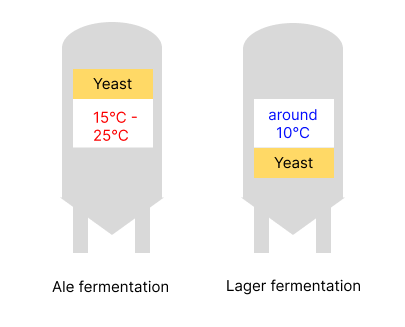
\includegraphics[scale=0.5]{images/beer_fermentation.png}
                \caption{Two types of beer fermentation}
                \small Temperature in Ale (Top) fermentation ideally is between 15°C to 25°C and temperature in Lager (bottom) fermentation ideally is between 6°C and 8°C which is colder compared to Ale fermentation\cite{viejo2019chemical}.
                \label{fig:intro:beer_fermentation}
            \end{figure}
                
            \paragraph*{Top fermentation}
                Top fermentation, also referred to as Ale Fermenting, entails introducing yeast directly onto the wort, where it starts fermenting from the top down. The yeast employed in ale fermentation is \textit{Saccharomyces cerevisiae}, which is also utilized in wine and bread making. 
                
                The ideal fermentation temperature for ale ranges from 15°C to 25°C. Most yeast types perish if the temperature exceeds 40°C \cite{viejo2019chemical}. The yeast used in lager fermentation can tolerate higher alcohol concentrations, which is why top-fermented beers generally have higher alcohol content than bottom-fermented beers. This yeast accelerates the fermentation process, allowing ale to be ready for consumption within a week. In general, top-fermented beers exhibit more robust flavors.

            \paragraph*{Bottom fermentation}
                In bottom fermentation or Lager Fermenting, the yeast in the wort starts working from the bottom up. The yeast typically employed for lager fermentation is \textit{Saccharomyces uvarum}. The optimal temperature range for lager fermentation lies between 6°C and 8°C \cite{viejo2019chemical}.

                Lager yeast becomes inactive when alcohol content surpasses a certain threshold, resulting in lager generally having a lower alcohol content than ale. The fermentation process is considerably slower than that of top fermentation beers, yielding a clearer and more refreshing beer.
                
            \paragraph*{Spontaneous fermentation}
                Spontaneous fermentation is an ancient and natural method of beer production, harnessing the power of wild, ambient microorganisms, predominantly yeast, and lactic acid bacteria, to convert the fermentable sugars in the wort into alcohol, carbon dioxide, and various flavor compounds. This uncontrolled and serendipitous process relies on the unique microbial ecosystem of a given environment, imparting distinctive, complex, and often unpredictable flavors to the resulting beer. The most notable example of spontaneously fermented beer is the Belgian Lambic, a sour and wild-fermented ale that reflects the rich microbiota of the Senne River Valley\cite{spitaels2014microbial}. Spontaneous fermentation is revered for its ability to capture the essence of a specific terroir and its innate capacity to produce unparalleled flavor profiles. However, due to the uncontrollable nature of wild microorganisms, the process can yield inconsistent results and may require lengthy maturation periods.

                While wild yeast, lactic acid bacteria (LAB), and certain other bacteria are typically deemed contaminants in many beer fermentation procedures, these same microorganisms are often desired in the crafting of specific sour beers and wild beer styles. Currently, the international beer market is witnessing a renewed interest in sour beers, as breweries of various sizes globally are exploring new product varieties and complex flavors\cite{bossaert2021description}. For instance, American Coolship Ales, a beer undergoing a complex series of spontaneous fermentations, is gaining popularity for its distinctive flavor profile\cite{bokulich2012brewhouse}. 
                
                This trend underscores the role of these traditionally "undesirable" microorganisms in creating novel and intriguing brews. More and more interest has been focused on identifying these microorganisms.
                
            \paragraph*{Non-spontaneous fermentation}
                In contrast, non-spontaneous fermentation is a controlled and deliberate process that employs selected strains of yeast and, occasionally, bacteria to ferment the wort. This method allows brewers to manipulate various parameters such as fermentation temperature, yeast strain, and wort composition, thereby enabling the production of a vast array of beer styles with consistent and reproducible characteristics. Non-spontaneous fermentation is the predominant method used in modern brewing, given its capacity for precision and the ability to tailor specific flavor profiles to cater to consumer preferences. Examples of beers produced through non-spontaneous fermentation include lagers, and ales, each showcasing distinct flavors and attributes attributed to the particular yeast strains employed and the conditions under which fermentation occurs\cite{white2010yeast}.
    
    
        \subsubsection{Beer microbiome studies overview}
            In this thesis, we have picked five studies related to beer microbiome analysis. Investigating these previous studies is beneficial for our beer microbiome analysis because it allows us to identify and understand the microbial compositions documented in earlier research and we can identify common trends and patterns. By reproducing the results using the data from the studies and comparing them with the original results, we can have a better understanding of our workflows' capability and performance. Among these, we have chosen to focus in detail on three studies that exhibited a higher variety of beers analyzed and were also among the most recent. They are BeerDeCoded: the open beer metagenome project\cite{sobel2017beerdecoded}, Bacterial and Fungal Dynamics During the Fermentation Process of Sesotho, a Traditional Beer of Southern Africa\cite{cason2020bacterial}, Characteristics of bacterial and yeast microbiomes in spontaneous and mixed-fermentation beer and cider \cite{tyakht2021characteristics}, A Culture-Independent Comparison of Microbial Communities of Two Maturating Craft Beers Styles\cite{costa2022culture} and Description of the temporal dynamics in microbial community composition and beer chemistry in sour beer production via barrel aging of finished beers \cite{bossaert2021description}. 3 of the 5 studies mentioned had a higher variety of beers, so they are discussed in detail here.
            
            \paragraph*{BeerDeCoded: the open beer metagenome project}
                The BeerDeCoded project analyzed the targeted metagenomic profile of 39 bottled beers using ITS sequencing of fungal species. These 39 commercial beers originated from 5 different European countries: 30 were from Switzerland, five from Belgium, two from Italy, one from France, and one from Austria.

                After extraction and sequencing the ITSs, a refined set of ITS sequences from the RefSeq database\cite{o2016reference} (Targeted Loci) was utilized to construct an ITS index for the \tool{Burrows-Wheeler Aligner (BWA)} \cite{li2009fast}. Using standard parameters, the \tool{BWA} was applied to align the beer sample reads, which are stored in \tool{FASTQ} format to this ITS index. Subsequently, the files were sorted and indexed using \tool{samtools} \cite{danecek2021twelve}. These BAM files underwent a quality control assessment with the aid of \tool{SAMstat}\cite{lassmann2011samstat}. To ensure accuracy and to remove low-quality, non-uniquely mapped reads, a minimum mapping quality (MAPQ) score of 3 was set as the threshold. Following this, the count of ITS per beer and per species was calculated, with only species having more than 10 reads considered for further analysis.
                
                The analysis revealed 42 distinct fungal species, intriguingly, 24 of these species were exclusive to just one type of beer. The extensive diversity of wild yeasts present in commercial beers was unanticipated, with some beers exhibiting evidence of containing over 10 different fungal species.
                
                Waldbier 2014 Schwarzkiefer, an Austrian beer incorporating pine cones sourced from local forests in its brewing process, stood out with the highest internal transcribed spacer (ITS) diversity, comprising 19 fungal species. In addition, two other beers both showed over 12 fungal species: La Nébuleuse Cumbres Rijkrallpa, a sour/wild ale that incorporates cranberries and fermented corn known as "Chicha", and Chimay Red Cap, a traditional Belgian Trappist beer.
                
            \paragraph*{Bacterial and Fungal Dynamics During the Fermentation Process of Sesotho, a Traditional Beer of Southern Africa}
                Sesotho, a widely consumed spontaneously fermented beer in Lesotho, Southern Africa, is brewed from milled maize, sorghum, or wheat flour, sometimes a blend of these. This beer is recognized for its cloudy appearance, light body, and characteristic sour taste. The goal of this study was to scrutinize the microbial diversity, covering both bacterial and fungal species, across five distinct stages of Sesotho fermentation. This was done at five unique locations in Lesotho, using Next-Generation Sequencing (NGS) methodologies.
                
                Ensuring data integrity and precision, all data sets underwent initial processing and trimming, with the aim of achieving an average quality score of at least 20. Sequences shorter than 200 base pairs were excluded. Subsequently, paired-end reads were amalgamated. A demultiplexing and quality filtering script in \tool{QIIME} was executed with default parameters, producing a FASTA output file. Chimeric sequences, or abnormal sequences composed of two distinct sequences, were recognized and removed. Then representative Operational Taxonomic Units (OTUs) were taxonomically classified, adhering to a 97\% sequence identity standard against the SILVA 132 database for the 16S rRNA bacterial data, and the UNITE database for the fungal ITS data.
                
                For the bacterial results, 9,885 bacterial OTUs were identified, with individual samples containing between 600 and 2,543 OTUs. \textit{Proteobacteria} and \textit{Firmicutes} emerged as the dominant bacterial phyla across all samples and locations. Regarding fungi, 46 OTUs were detected at the same sequencing depth across all samples, with individual samples yielding between 5 and 13 OTUs. The prevailing fungal phyla across all samples and locations were \textit{Ascomycota} and \textit{Mucoromycota}, with \textit{Saccharomyces spp}. being an example of the Ascomycota. This research offers valuable insights into the microbial ecology involved in Sesotho beer fermentation.
                
            \paragraph*{Characteristics of bacterial and yeast microbiomes in spontaneous and mixed-fermentation beer and cider}
                This study concentrates on the microbial communities within 14 commercially available Russian beers, known for their mixed or spontaneous fermentation. These beer samples were either acquired from retail stores or directly supplied by the manufacturers. The analysis hinged on High Throughput Sequencing of 16S rRNA and ITS regions from these beer samples.

                The data was processed utilizing the \tool{Knomics-Biota system}, which was enhanced by authors to scrutinize the prokaryotic and yeast microbiomes associated with food products. Firstly, the reference databases were expanded to accommodate 16S rRNA sequencing data from any niche. Secondly, a new module was incorporated for analyzing the fungal ITS region. This module is based on the UNITE database \cite{nilsson2019unite}, utilizes the Deblur algorithm \cite{amir2017deblur} for amplicon-sequence variant (ASV) identification, and employs the \tool{QIIME2 naive-Bayes classifier}.
                
                Given the diversity in the samples, which encompassed mixed-fermentation beer, it was anticipated that the yeast composition would not be restricted to \textit{Saccharomyces cerevisiae}. As hypothesized, the microbiome was primarily influenced by the balance between \textit{Dekkera} (also known as \textit{Brettanomyces}) and \textit{Saccharomyces}, while other less prevalent contributors included \textit{Issatchenkia}, \textit{Pichia}, \textit{Hanseniaspora}, and \textit{Candida}. On a species level, \textit{Dekkera} was predominantly represented by \textit{D. bruxellensis}, with minor presence of \textit{D. custersiana} and \textit{D. anomala}. \textit{Saccharomyces} was chiefly represented by \textit{S. cerevisiae} and \textit{S. bayanus/pastorianus} among others. On the other hand, the bacterial community was predominantly composed of members from the \textit{Lactobacillales} order. Other bacterial families were generally found in low abundances in the beer samples, except for three instances where the \textit{Enterobacteriaceae}, \textit{Leuconostocaceae}, and \textit{Acetobacteraceae} families were present in considerable (>5\%) quantities.

            \paragraph*{Summary of prior beer microbiome studies}
                These 3 studies focus on different types of beer, but all studies employ metagenomic profiling, targeting fungal ITS and bacterial 16S rRNA regions, to investigate the microbial communities in beers. And the studies utilize similar data analysis steps just like discussed previously, such as quality control, taxonomic profiling, and diversity analysis \& visualization. Across the studies, the predominant fungal phylum observed is \textit{Ascomycota}, within which \textit{Saccharomyces spp}. are identified as key contributors to the beer microbiome. This genus is known for its pivotal role in the fermentation process. The studies report \textit{Proteobacteria} and \textit{Firmicutes} as dominant bacterial phyla, with members of the \textit{Lactobacillales} order frequently detected. These bacteria are responsible for the production of lactic acid and other metabolites that impact beer flavor profiles.
                